\chapter{Analyse}

I dette kapitel vil vi gennemgå kravspecifikation til programmet, samt optegne og forklare forskellige modeller.


\section{Kravspecifikation}

Herunder ses en liste over krav til spillet, udformet udfra opgavebeskrivelsen.\footnote{Enkelte krav er hentet fra tidligere CDIO2-rapport af samme gruppe.}

\begin{enumerate}
\item Spillet skal være en viderebygning på det tidligere udviklet spil fra CDIO 2.
\item Man skal kunne spille 2-4 spillere.
\item Der skal implementeres væsentlige elementer fra Monopoly Junior.
\item Der skal oprettes forskellige typer felter, samt en spilleplade.
\item Hvert felt skal påvirke spillernes pengebeholdning forskelligt, og have en udskrift om hvilket felt han ramte.
\item Spillerne skal kunne lande på et felt, og fortsætte derfra på næste slag.
\item Spillerne skal gå i ring rundt på felterne, på spillepladen.
\item Spillet skal kunne køre på DTU's databar-computere.
\item Der skal implementeres med regler fra et rigtigt Monopoly Junior spil.
\end{enumerate}

\pagebreak

\subsection{FURPS+ \& MoSCoW}

\subsubsection{FURPS+}

FURPS+ er en metode til at kategorisere / klassificere krav. \\
Vi har i denne opgave brugt FURPS+ metoden til at kategorisere de krav, som er udformet fra opgavebeskrivelsen.
Vi har ikke valgt at medtage alle FURPS+ punkterne, men medbragt dem der giver mening for opgaven. \\
Herunder ses et eksempel på FURPS+, og hvad de enkelte kategorier kan indeholde.\footnote{FURPS+ tabellen der vises, er hentet fra tidligere CDIO2-rapport af samme gruppe.}

\begin{figure*}[ht]{
    \centering
\begin{tabular}{|c | p{0,05cm} p{2,8cm} |p{10,5cm}|}
       \hline
       \textbf{F}   &   Functionality   &&
       Egenskaber, ydeevne, sikkerhed                   \\
       \hline

       \textbf{U}   &   Usability       &&
       Menneskelige faktorer, hjælp, dokumentation      \\
       \hline

       \textbf{R}   &   Reliability     &&
       Fejlfrekvens, fejlretning, forudsigelighed       \\
       \hline

       \textbf{P}   &   Performance     &&
       Svartider, nøjagtighed, ydeevne, ressourceforbrug                                                      \\
       \hline

       \textbf{S}   &   Supportability  &&
       Anvendelighed, tilpasningsevne, vedligeholdbarhed                                                      \\
       \hline

       \textbf{+}   &                   &&              \\

       &&   Implementation: &   Ressourcebegrænsninger, sprog og værktøjer, hardware                     \\

       &&   Interface:      &   Begrænsninger forårsaget af kommunikation med eksterne systemer              \\

       &&   Operations:     &   Systemstyring i dets operationelle ramme                              \\

       &&   Packaging:      &   F.eks. en fysisk boks   \\

       &&    Legal:         &   F.eks. licenser       \\
       \hline
\end{tabular}}
\end{figure*}

\noindent Vi her herunder en oversigt over krav til opgaven, kategoriseret ved hjælp af FURPS+.
\\\\\textbf{Functionality:}\\
1. Spillet skal være en viderebygning på det tidligere udviklet spil fra CDIO 2.
6. Spillerne skal kunne lande på et felt, og fortsætte derfra på næste slag.
4. Der skal oprettes forskellige typer felter, samt en spilleplade.
5. Hvert felt skal påvirke spillernes pengebeholdning forskelligt, og have en udskrift om hvilket felt han ramte.
9. Der skal implementeres med regler fra et rigtigt Monopoly Junior spil.
\\\\\textbf{Usability:}\\
2. Man skal kunne spille 2-4 spillere.
\\\\\textbf{(+) - Implementation:}\\
8. Spillet skal kunne køre på DTU's databar-computere.
\\\\\textbf{(+) - Interface:}\\
7. Spillerne skal gå i ring rundt på felterne, på spillepladen.
5. Hvert felt skal påvirke spillernes pengebeholdning forskelligt, og have en udskrift om hvilket felt han ramte.

\pagebreak

\subsubsection{MoSCoW}

MoSCoW, er et værktøj som kan bruges til at prioritere krav.
Herunder ses et eksempel på MoSCoW, og hvad de enkelte kategorier kan indeholde.\footnote{MoSCoW tabellen der vises, er hentet fra tidligere CDIO2-rapport af samme gruppe.} \\\\

\begin{tabular}{lll}
    \textbf{Mo} &   
    "Must have"                 &
    De mest vitale krav, vi ikke kan undgå. \\

    \textbf{S}  &   
    "Should have"               & 
    Vigtige krav, som ikke er vitale. \\

    \textbf{Co} &   
    "Could have"                & 
    The 'nice-to-haves' \\

    \textbf{W}  &   
    "Won’t have (this time)"    & 
    Things that provide little to no value you can give up on \\

\end{tabular}
\\\\

\noindent Vi her herunder en oversigt over krav til opgaven, prioriteret ved hjælp af MoSCoW.

\begin{center}
    \begin{tabular}{ | l | p{13cm} |}
    \hline
    \textbf{Must have}
    &        
        2. Man skal kunne spille 2-4 spillere.

        4. Der skal oprettes forskellige typer felter, samt en spilleplade.
        
        6. Spillerne skal kunne lande på et felt, og fortsætte derfra på næste slag.
        
        8. Spillet skal kunne køre på DTU’s databar-computere.
    \\
    
    \hline
    \textbf{Should have}
    &
        1. Spillet skal være en viderebygning på det tidligere udviklet spil fra CDIO 2.

        3. Der skal implementeres væsentlige elementer fra Monopoly Junior.

        5. Hvert felt skal påvirke spillernes pengebeholdning forskelligt, og have en ud-skrift om hvilket felt han ramte.

        7. Spillerne skal gå i ring rundt på felterne, på spillepladen.
    \\
    \hline
    \textbf{Could have}
    &
        9. Der skal implementeres med regler fra et rigtigt Monopoly Junior spil.
    \\
    \hline
    \textbf{Won't have}
    &

    \\
    \hline
    \end{tabular}
\end{center}

\noindent Vi har ikke nogen krav der kan sættes i kategorien won't have.
Dette felt bruges ofte til krav der bliver stillet fra kunden, som man ikke kan udføre, eller har svært ved pga. ressourcer eller lign.
Der er selvfølgelig plads til videreudvikling i vores, hvilket ville ligge under won't have. 

\section{Interessentanalyse}

    \begin{tabular}{ | l | p{13cm} |}
    \hline
    \textbf{Interresent} & \textbf{Interesse / Mål} \\ \hline
    Spiller/-e & Kunne styre et system, der styrer et spil mellem 2-4 personer, 
    hvor i der kastes en terning, og man ser resultatet af dette slag med det samme, herefter skal facevaluen af dette slag fortælle, hvilket felt spilleren landte på, derudover skal den kunne fortælle om feltet er ejet, eller om det er frit til at købe, således at man enten skal betale til en spiller, eller har mulighed for at købe grunden.\\ \hline
    \hline
    \end{tabular}


\newpage

\section{Use case}

Følgende er en liste over use cases samt deres beskrivelser i en fully dressed udgave.

%\footnote{Use case modellen i tabel 3.1 er en revideret udgave af use case modellen fra CDIO 1 da vi har at gøre med en magen til konfiguration.}

\begin{table}[H]
    \begin{center}
        \begin{tabular}{ | p{15cm} |}
            \hline
            \textbf{Use case:} PlayGame \\ \hline
            \textbf{ID:} UC1 \\ \hline
            \textbf{Brief description} Spiller/-e skal kunne spille spil/Game (starte spillet) og slå med to terninger     \\ \hline
            \textbf{Primary actors:} Spiller/-e \\ \hline
            \textbf{Secondary actors:} Ingen. \\ \hline
            \textbf{Preconditions:} Ingen.     \\ \hline
            \textbf{Main flow:}
            \begin{enumerate}
                \item \textbf{Antal spillerer indtastes (minimum 2 og maksimum 6 spillerer) og tildeles 30.000 i pengebeholdning.}
                \item \textbf{Spillerer slår med to terninger, lander på et felt mellem 1-21 og bliver udefra det tildelt en opdateret pengebeholdning.}
                \item \textbf{Spillet slutter når alle, på nær én spiller, er bankerot.}
            \end{enumerate} \\ \hline
            \textbf{Postconditions:} Ingen.\\ \hline
            \textbf{Alternative flow:} Ingen.\\ \hline
            \hline
        \end{tabular}
        \caption{Use case 1}
        \label{usecase:1}
    \end{center}
\end{table}

\begin{table}[H]
    \begin{center}
        \begin{tabular}{ | p{15cm} |}
            \hline
            \textbf{Use case:} Fleet: Not owned, no intention to buy \\ \hline
            \textbf{ID:} UC2 \\ \hline
            \textbf{Brief description} I tilfælde af at spiller/-e lander på et felt som hverken ejes eller har intention om at købe.     \\ \hline
            \textbf{Primary actors:} Spiller/-e \\ \hline
            \textbf{Secondary actors:} Ingen. \\ \hline
            \textbf{Preconditions:}
            \\- Navn på spillerer er registreret
            \\- Terningerne er slået \\ \hline
            \textbf{Main flow:}
            \begin{enumerate}
                \item \textbf{Spiller lander på felt.}
                \item \textbf{Med udgangspunkt i brugerinteraktion med GUI, afgører spiller hvorledes der ønskes, at købe felt eller springe over.}
                \item \textbf{I denne usecase, takker spiller nej til køb af felt.}
            \end{enumerate} \\ \hline
            \textbf{Postconditions:} Spillet fortsætter og turen går til næste spiller.\\ \hline
            \textbf{Alternative flow:}
            \\- UC3: Fleet: Owned
            \\- UC4: Fleet: Not owned, intention to buy\\ \hline
            \hline
        \end{tabular}
        \caption{Use case 2}
        \label{usecase:2}
    \end{center}
\end{table}

\begin{table}[H]
    \begin{center}
        \begin{tabular}{ | p{15cm} |}
            \hline
            \textbf{Use case:} Fleet: Owned \\ \hline
            \textbf{ID:} UC3 \\ \hline
            \textbf{Brief description} I tilfælde af at spiller/-e lander på et felt som er ejet.    \\ \hline
            \textbf{Primary actors:} Spiller/-e \\ \hline
            \textbf{Secondary actors:} Ingen. \\ \hline
            \textbf{Preconditions:}
            \\- Navn på spillerer er registreret
            \\- Terningerne er slået \\ \hline
            \textbf{Main flow:}
            \begin{enumerate}
                \item \textbf{Spiller lander på felt.}
                \item \textbf{Spillet fremviser vha. GUI detaljer om feltet til spiller, herunder om feltet er ejet, og af hvem samt det beløb der skal trækkes fra den berørte spillers pengebeholdning.}
                \item \textbf{Der bliver trukket i spillerens pengebeholdning, undtagelsesvis hvis spillers pengebeholdning går i minus, og erklæres hermed bankerot.}
            \end{enumerate} \\ \hline
            \textbf{Postconditions:} Spillet fortsætter og turen går til næste spiller.\\ \hline
            \textbf{Alternative flow:}
            \\- UC2: Fleet: Fleet: Not owned, no intention to buy
            \\- UC4: Fleet: not owned, intention to buy.\\ \hline
            \hline
        \end{tabular}
        \caption{Use case 3}
        \label{usecase:3}
    \end{center}
\end{table}

\begin{table}[H]
    \begin{center}
        \begin{tabular}{ | p{15cm} |}
            \hline
            \textbf{Use case:} Fleet: Not owned, intention to buy \\ \hline
            \textbf{ID:} UC4 \\ \hline
            \textbf{Brief description} I tilfælde af at spiller/-e lander på et felt som ikke ejes, men har intention om at købe.    \\ \hline
            \textbf{Primary actors:} Spiller/-e \\ \hline
            \textbf{Secondary actors:} Ingen. \\ \hline
            \textbf{Preconditions:}
            \\- Navn på spillerer er registreret
            \\- Terningerne er slået \\ \hline
            \textbf{Main flow:}
            \begin{enumerate}
                \item \textbf{Spiller lander på felt.}
                \item \textbf{Med udgangspunkt i brugerinteraktion med GUI, afgører spiller hvorledes der ønskes, at købe felt eller springe over.}
                \item \textbf{I denne usecase, takker spiller ja til køb af felt.}
                \item \textbf{Der bliver trukket i spillerens pengebeholdning, undtagelsesvis hvis spillers pengebeholdning går i minus, og erklæres hermed bankerot.}
            \end{enumerate} \\ \hline
            \textbf{Postconditions:} Spiller tildeles købt felt, spillet fortsætter og turen går til næste spiller.\\ \hline
            \textbf{Alternative flow:}
            \\- UC2: Fleet: Not owned, no intention to buy
            \\- UC3: Fleet: Owned.\\ \hline
            \hline
        \end{tabular}
        \caption{Use case 4}
        \label{usecase:4}
    \end{center}
\end{table}

\subsection{Use case diagram}
Use cases bliver lavet for at skabe overblik over det kommende program.
Ligeledes har vi valgt at inddrage et use case-diagram for at illustrere, hvordan det ser ud for vores program.
Use case-diagrammet er meget beskedent, idet der kun er én aktør, nemlig spilleren, som kun kan gøre én ting, nemlig at spille spillet.
\begin{figure}[H]
    \begin{center}
        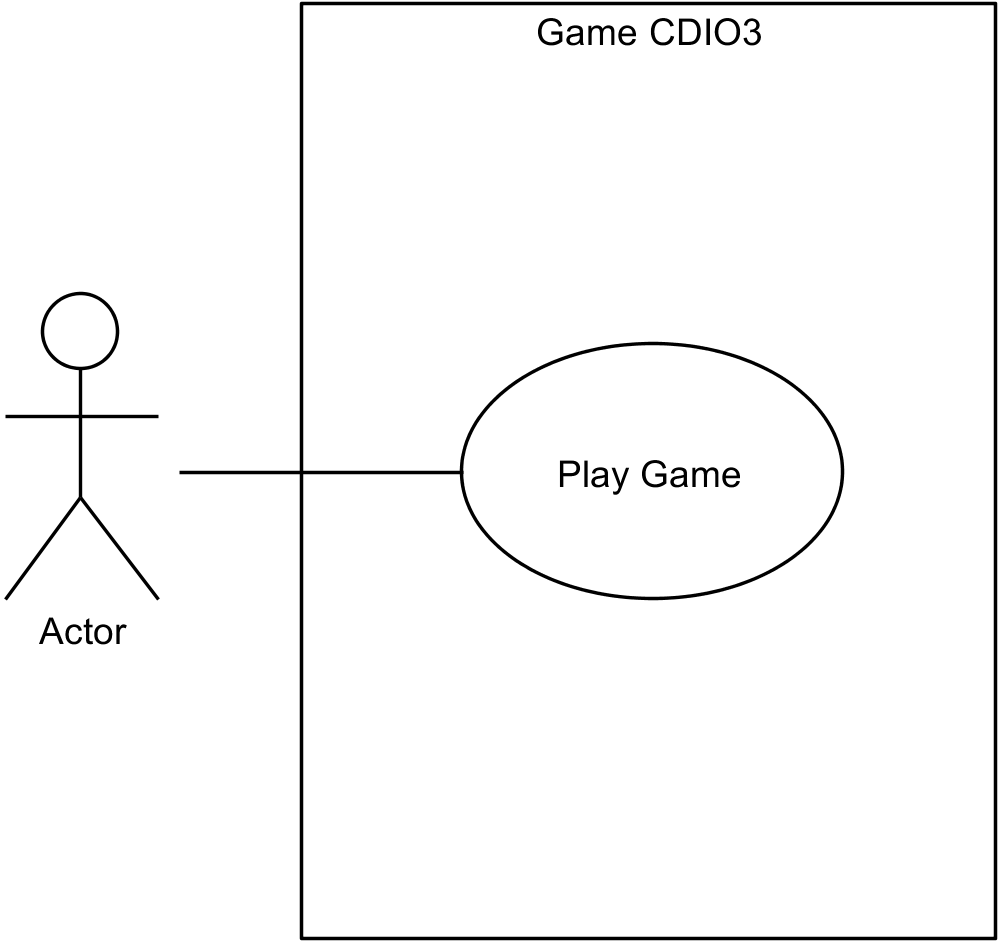
\includegraphics[width=8cm]{graphics/usecases/UseCase1.png}
        \caption{Use case diagram}
        \label{fig:use_case_diagram}
    \end{center}
\end{figure}

\pagebreak
\section{Domænemodel}